\documentclass{report}
\usepackage{hyperref}
\hypersetup{
    colorlinks=true,
    linkcolor=blue,
    filecolor=magenta,      
    urlcolor=cyan,
}
\usepackage{graphicx}
\graphicspath{ {imagenes/} }
\usepackage[utf8]{inputenc}
\makeatletter
\usepackage{color}
\definecolor{lightgray}{rgb}{0.95, 0.95, 0.95}
\definecolor{darkgray}{rgb}{0.4, 0.4, 0.4}
%\definecolor{purple}{rgb}{0.65, 0.12, 0.82}
\definecolor{editorGray}{rgb}{0.95, 0.95, 0.95}
\definecolor{editorOcher}{rgb}{1, 0.5, 0} % #FF7F00 -> rgb(239, 169, 0)
\definecolor{editorGreen}{rgb}{0, 0.5, 0} % #007C00 -> rgb(0, 124, 0)
\definecolor{orange}{rgb}{1,0.45,0.13}		
\definecolor{olive}{rgb}{0.17,0.59,0.20}
\definecolor{brown}{rgb}{0.69,0.31,0.31}
\definecolor{purple}{rgb}{0.38,0.18,0.81}
\definecolor{lightblue}{rgb}{0.1,0.57,0.7}
\definecolor{lightred}{rgb}{1,0.4,0.5}
\usepackage{upquote}
\usepackage{listings}
% CSS
\lstdefinelanguage{CSS}{
  keywords={color,background-image:,margin,padding,font,weight,display,position,top,left,right,bottom,list,style,border,size,white,space,min,width, transition:, transform:, transition-property, transition-duration, transition-timing-function},	
  sensitive=true,
  morecomment=[l]{//},
  morecomment=[s]{/*}{*/},
  morestring=[b]',
  morestring=[b]",
  alsoletter={:},
  alsodigit={-}
}

% JavaScript
\lstdefinelanguage{JavaScript}{
  morekeywords={typeof, new, true, false, catch, function, return, null, catch, switch, var, if, in, while, do, else, case, break},
  morecomment=[s]{/*}{*/},
  morecomment=[l]//,
  morestring=[b]",
  morestring=[b]'
}

\lstdefinelanguage{HTML5}{
  language=html,
  sensitive=true,	
  alsoletter={<>=-},	
  morecomment=[s]{<!-}{-->},
  tag=[s],
  otherkeywords={
  % General
  >,
  % Standard tags
	<!DOCTYPE,
  </html, <html, <head, <title, </title, <style, </style, <link, </head, <meta, />,
	% body
	</body, <body,
	% Divs
	</div, <div, </div>, 
	% Paragraphs
	</p, <p, </p>,
	% scripts
	</script, <script,
  % More tags...
  <canvas, /canvas>, <svg, <rect, <animateTransform, </rect>, </svg>, <video, <source, <iframe, </iframe>, </video>, <image, </image>, <header, </header, <article, </article
  },
  ndkeywords={
  % General
  =,
  % HTML attributes
  charset=, src=, id=, width=, height=, style=, type=, rel=, href=,
  % SVG attributes
  fill=, attributeName=, begin=, dur=, from=, to=, poster=, controls=, x=, y=, repeatCount=, xlink:href=,
  % properties
  margin:, padding:, background-image:, border:, top:, left:, position:, width:, height:, margin-top:, margin-bottom:, font-size:, line-height:,
	% CSS3 properties
  transform:, -moz-transform:, -webkit-transform:,
  animation:, -webkit-animation:,
  transition:,  transition-duration:, transition-property:, transition-timing-function:,
  }
}

\lstdefinestyle{htmlcssjs} {%
  % General design
%  backgroundcolor=\color{editorGray},
  basicstyle={\footnotesize\ttfamily},   
  frame=b,
  % line-numbers
  xleftmargin={0.75cm},
  numbers=left,
  stepnumber=1,
  firstnumber=1,
  numberfirstline=true,	
  % Code design
  identifierstyle=\color{black},
  keywordstyle=\color{blue}\bfseries,
  ndkeywordstyle=\color{editorGreen}\bfseries,
  stringstyle=\color{editorOcher}\ttfamily,
  commentstyle=\color{brown}\ttfamily,
  % Code
  language=HTML5,
  alsolanguage=JavaScript,
  alsodigit={.:;},	
  tabsize=2,
  showtabs=false,
  showspaces=false,
  showstringspaces=false,
  extendedchars=true,
  breaklines=true,
  % German umlauts
  literate=%
  {Ö}{{\"O}}1
  {Ä}{{\"A}}1
  {Ü}{{\"U}}1
  {ß}{{\ss}}1
  {ü}{{\"u}}1
  {ä}{{\"a}}1
  {ö}{{\"o}}1
}
%
\lstdefinestyle{py} {%
language=python,
literate=%
*{0}{{{\color{lightred}0}}}1
{1}{{{\color{lightred}1}}}1
{2}{{{\color{lightred}2}}}1
{3}{{{\color{lightred}3}}}1
{4}{{{\color{lightred}4}}}1
{5}{{{\color{lightred}5}}}1
{6}{{{\color{lightred}6}}}1
{7}{{{\color{lightred}7}}}1
{8}{{{\color{lightred}8}}}1
{9}{{{\color{lightred}9}}}1,
basicstyle=\footnotesize\ttfamily, % Standardschrift
numbers=left,               % Ort der Zeilennummern
%numberstyle=\tiny,          % Stil der Zeilennummern
%stepnumber=2,               % Abstand zwischen den Zeilennummern
numbersep=5pt,              % Abstand der Nummern zum Text
tabsize=4,                  % Groesse von Tabs
extendedchars=true,         %
breaklines=true,            % Zeilen werden Umgebrochen
keywordstyle=\color{blue}\bfseries,
frame=b,
commentstyle=\color{brown}\itshape,
stringstyle=\color{editorOcher}\ttfamily, % Farbe der String
showspaces=false,           % Leerzeichen anzeigen ?
showtabs=false,             % Tabs anzeigen ?
xleftmargin=17pt,
framexleftmargin=17pt,
framexrightmargin=5pt,
framexbottommargin=4pt,
%backgroundcolor=\color{lightgray},
showstringspaces=false,      % Leerzeichen in Strings anzeigen ?
}%
%
\makeatother

\begin{document}
\begin{titlepage}
    \centering
    {\bfseries\LARGE Universidad Politécnica Salesiana \par}
    \vspace{1cm}
    {\scshape\Large Ingeniería en Ciencias de la Computación \par}
    \vspace{3cm}
    {\scshape\Huge APLICACIÓN DEL CLIMA \par}
    \vspace{1cm}
    {\center
\includegraphics[width=5cm, height=5cm]{ups1.png}\\}
    \vspace{1cm}
    {\itshape\Large Informe 03 \par}
    \vfill
    {\Large Autor: \par}
    {\Large Ricardo Romo \par}
    \vfill
    {\Large \today \par}
    \end{titlepage} 
    \textbf{PROBLEMA}   
    \\
    Se desea crea una aplica la cual reciba los parámetros de -c (ciudad a la cual se desea sacar la información), -o (opciones p=presión , h=humedad, su demanda no es necesaria), y la cual muestre por consola, La ciudad, la temperatura de esta, si se envía el parámetro -o p se mostrara la presión y si es -o h la humedad, para realizar este proceso deberá conectarse a una API
    Antes de comenzar lo primero que debemos de hacer es crearnos una cuanta dentro de \textbf{Rapid API} \url{https://rapidapi.com/}
    \begin{center}
        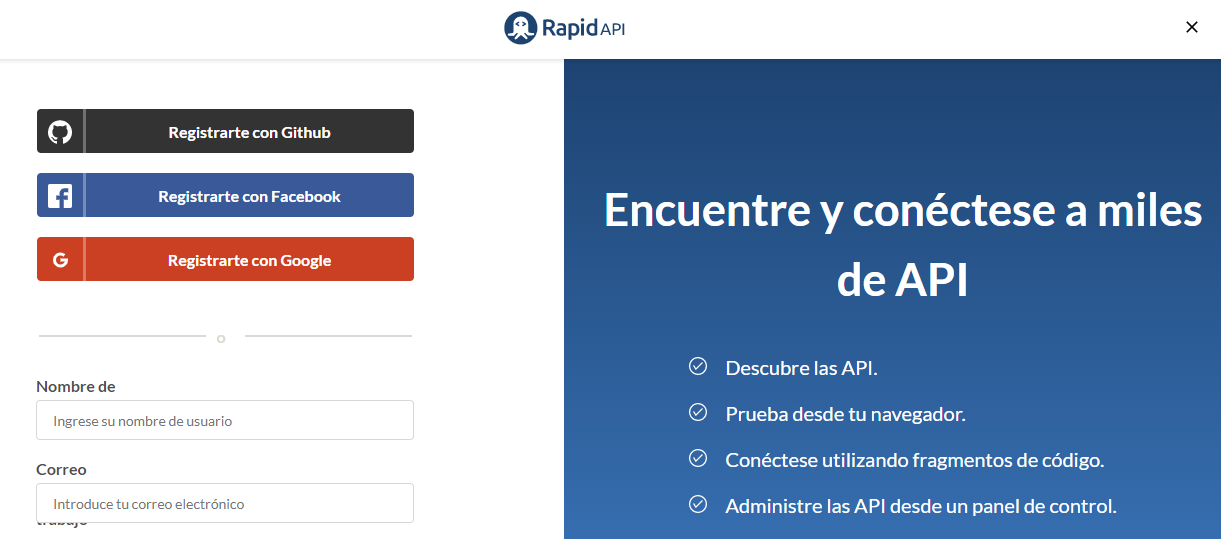
\includegraphics[scale=0.5]{rapid.PNG}
      \end{center}
    Luego iniciamos sesión y nos dirigimos a la API de \textbf{ Open Weather Map} \url{https://rapidapi.com/community/api/open-weather-map}, esta API nos en entrega en tiempo real la temperatura, presión, humedad, entre otros datos
    sobre una ciudad que se elija, este mismo api nos entra un identificador el cual nos servirá para hacer peticiones a esta API.
    \begin{center}
        
\includegraphics[scale=0.9]{key.PNG}
      \end{center}
      Y ya con esto podemos comenzar
    \begin{enumerate}
        \item Comenzamos iniciando npm con los comandos \textbf{npm init}
        \item Luego instalamos nuestras dependencias que en este caso usaremos las siguientes:
        \begin{enumerate}
            \item \textbf{npm install axios \-\-save}
            \item \textbf{npm install yargs \-\-save}
        \end{enumerate}
    \end{enumerate}
    Una vez ya instaladas nuestras dependencias proseguimos a crea una carpeta llamada controlador y dentro de esta un archivo llamado \textbf{clima.js}.
    Este \textbf{clima.js} va a ser nuestro controlador, es decir va a realizar los pedidos a la API.
    \\
    \textbf{clima.js}
    \begin{enumerate}
        \item Primero llamamos a nuestro modulo Axios con el comando require
        \item Creamos la función asyn getClima() el cual recibiremos el nombre de la ciudad, y la opción de los datos que se necesita siendo p para presión y h para humedad.
        \item Utilizamos el comando \textbf{encodeURI} para codificar la ciudad en modo URL para que la petición get pueda procesarla
        \item Llamamos a nuestro modulo axios.get() para realizar una petición tipo get enviando como parámetros nuestra \textbf{key} proporcionada por la API en la página \textbf{appid} y la ciudad que deseamos consultar la información \textbf{q}
        \item Una vez obtenidos los resultamos guardamos en un objeto y retornamos dependiendo la respuesta que necesitemos
        \item Por último exportamos esta función con \textbf{module.exports}
    \end{enumerate}
    \lstinputlisting[firstline=1,lastline=17,style=htmlcssjs]{codigo/controlador/clima.js}
   %-----------------------------------
   Ahora crearemos en la carpeta raíz nuestro main que lo nombraremos como \textbf{app.js}
   \\
   \textbf{app.js}
   \\
   \begin{enumerate}
       \item Comenzamos llamando a nuestro modulo \textbf{yargs} con el comando require, seguido por el comando \textbf{.options} en el cual se enviaran todos los datos a ser ingresados por el usuario , en este caso sería \textbf{city,option}, teniendo cada uno su propia configuración, al final, enviamos .argv para recibir estos argumentos.
       \item Llamaremos también a nuestro controlador ya exportado y lo nombraremos como \textbf{weather}
       \item Crearemos una función asyn llamada get\_information(), el cual recibirá los parámetros de la ciudad.
       \item Creamos la variable values la cual recibirá de nuestro controlador \textbf{clima.js} los datos que se pidió.
       \item al final llamamos a la función get\_information(), enviamos la ciudad, e imprimimos la respuesta dentro de una tabla. 
   \end{enumerate}
   \lstinputlisting[firstline=1,lastline=27,style=htmlcssjs]{codigo/app.js}
   
   \textbf{EJECUCIÓN 1}
   \begin{center}
       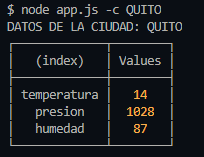
\includegraphics[scale=0.9]{ej1.PNG}
     \end{center}
   \textbf{EJECUCIÓN 2}
   \begin{center}
       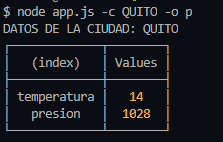
\includegraphics[scale=0.9]{ej2.PNG}
     \end{center}
     \textbf{EJECUCIÓN 3}
     \begin{center}
       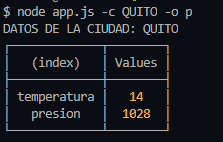
\includegraphics[scale=0.9]{ej3.PNG}
     \end{center}
   \textbf{CONCLUSIÓN}
   \begin{itemize}
       \item Las conexiones a APIS es un recurso necesario para los servicios web, debido a que estas dos se complementan, es decir la una obtiene información, y la otra procesa la información realizando las respectivas operaciones que desee el usuario.
   \end{itemize}
   
   \textbf{CÓDIGO}
   \\
   \url{https://github.com/rromom/clases-web/tree/master/codigos}
\end{document}